%!TEX TS-program = pdflatex
% dissertation.tex -- main dissertation file
%
% Wisconsin dissertation template
% Copyright (c) 2008-2009 William C. Benton.  All rights reserved.
%
% This program can redistributed and/or modified under the terms
% of the LaTeX Project Public License Distributed from CTAN
% archives in directory macros/latex/base/lppl.txt; either
% version 1 of the License, or (at your option) any later version.
%
% This program includes other software that is licensed under the
% terms of the LPPL and the Perl Artistic License; see README for details.
%
% You, the user, still hold the copyright to any document you produce
% with this software (like your dissertation).
%

%%% You'll want ``oneside'' for the deposit version, but probably not for any versions that don't need to meet the UW requirements
\documentclass[12pt,oneside,letterpaper]{memoir}

% preamble.tex -- packages to include
%
% Wisconsin dissertation template
% Copyright (c) 2008 William C. Benton.  All rights reserved.
%
% This program can redistributed and/or modified under the terms
% of the LaTeX Project Public License Distributed from CTAN
% archives in directory macros/latex/base/lppl.txt; either
% version 1 of the License, or (at your option) any later version.
%
% This program includes other software that is licensed under the
% terms of the LPPL and the Perl Artistic License; see README for details.
%
% You, the user, still hold the copyright to any document you produce
% with this software (like your dissertation).

%% You should use natbib
\IfFileExists{natbib.sty}{%
\usepackage[numbers,sort]{natbib}%
}{}

%% You probably need appendix, if you want appendices
\IfFileExists{appendix.sty}{%
\usepackage{appendix}%
}{}

%% the spacing in memoir is weird, you'll need to use this
\DisemulatePackage{setspace}
\usepackage[onehalfspacing]{setspace}

%% List setup; the ``hanglist`` environment will allow you to have
%% nicely-typeset enumerated lists (i.e. with the numbers hanging in
%% the margins).  You need at least version 2.1 of enumitem.sty.  If
%% you don't have enumitem installed at all, hanglist will just be an
%% alias for enumerate.
\IfFileExists{enumitem.sty}{%
\usepackage[loadonly]{enumitem}[2007/06/30]%
\newlist{hanglist}{enumerate}{1}% 
\setlist[hanglist]{label=\arabic*.}%
\setlist[hanglist,1]{leftmargin=0pt}%
}{%
\newenvironment{hanglist}{\begin{enumerate}}{\end{enumerate}}%
}

%% Comment out any of these that you don't want
\usepackage{amssymb}
\usepackage{amsmath}
\usepackage{amsthm}
%\usepackage{theorem}
\usepackage{hyperref}

\IfFileExists{mathpartir.sty}{%
\usepackage{mathpartir}%
}{}

%%%%% LISTINGS package and setup
\IfFileExists{listings.sty}{%
\usepackage{listings}%
}{}



%% Get rid of ugly borders around PDF hyperlinks (e.g. for cross-references, bib entries, or URLs)
\hypersetup{pdfborder = 0 0 0}

%% You want microtype.
\IfFileExists{microtype.sty}{%
\usepackage[protrusion=true,expansion=true]{microtype}%
}{}

%\pagestyle{thesisdraft}

% Surround parts of graphics with box
\usepackage{boxedminipage}

%% booktabs (thx to Nate Rosenblum for bringing this beautiful package
%% to my attention)
\IfFileExists{booktabs.sty}{%
\usepackage{booktabs}%
}{}

% This is now the recommended way for checking for PDFLaTeX:
\usepackage{ifpdf}

%% Avoid ugly "Type 3" fonts
\usepackage{lmodern}
\usepackage[LY1]{fontenc}

%% Substitute your favorite serif and sans fonts here....
\IfFileExists{tgpagella.sty}{%
% TeX Gyre pagella, like Palatino
\usepackage{tgpagella}%
}{}

\usepackage[LY1]{eulervm}

\ifpdf
\usepackage[pdftex]{graphicx}
\else
\usepackage{graphicx}
\fi

\usepackage{makeidx}
\makeindex

{\theoremstyle{plain}
\newtheorem{thm}{Theorem}[chapter]
\newtheorem{cor}[thm]{Corollary}
\newtheorem{define}[thm]{Definition}
\newtheorem{exmpl}[thm]{Example}
}
{\theoremstyle{remark}
\newtheorem{rmk}[thm]{Remark}
}

\newtheoremstyle{customsty1}
{3pt}%
{3pt}%
{}% --- body font
{}% --- indent amount
{\bfseries}% --- Theorem head font
{:}% --- Punctuation after head
{.5em}% --- space after head
{}% --- theorem head spec (can be left empty, meaning 'normal')

% Define 'newtheorems' that use ``customsty1''
{\theoremstyle{customsty1} 
}


%%% NB: the ``deposit'' chapter- and page- styles should conform to UW
%%% requirements.  If you are producing a pretty version of your
%%% dissertation for web use later, you will certainly want to make
%%% your own chapter and page styles.

\makechapterstyle{deposit}{%
  \renewcommand{\chapterheadstart}{}
  \renewcommand{\printchaptername}{}
  \renewcommand{\chapternamenum}{}
  \renewcommand{\printchapternum}{\parbox{2em}{\MakeLowercase{\Large\scshape\thechapter{}}} }
  \renewcommand{\afterchapternum}{}
  \renewcommand{\printchaptertitle}[1]{%
  \raggedright\Large\scshape\MakeLowercase{##1}}
  \renewcommand{\afterchaptertitle}{%
  \vskip\onelineskip \hrule\vskip\onelineskip}
}

\makepagestyle{deposit}
 
\makeatletter
 
\renewcommand{\chaptermark}[1]{\markboth{#1}{}}
\renewcommand{\sectionmark}[1]{\markboth{#1}{}}
 
\makeevenfoot{deposit}{}{}{}
\makeoddfoot{deposit}{}{}{}
\makeevenhead{deposit}{\thepage}{}{}
\makeoddhead{deposit}{}{}{\thepage}
\makeatother

%%% set up page numbering for chapter pages to satisfy UW requirements
%%% NB: You will want to delete until the ``SNIP'' mark if you are
%%% making a ``nice'' copy
\copypagestyle{chapter}{plain}
\makeoddfoot{chapter}{}{}{}
\makeevenhead{chapter}{\thepage}{}{}
\makeoddhead{chapter}{}{}{\thepage}
%%% SNIP

%%% bib nonsense
\makeatletter
\newenvironment{wb-bib}[1]{%
  \chapter*{references}
\ifnobibintoc\else 
\phantomsection 
\addcontentsline{toc}{chapter}{References} 
\fi 
\prebibhook
  \begin{bibitemlist}{#1}}{\end{bibitemlist}\postbibhook}

\AtBeginDocument{%
  \@ifpackageloaded{natbib}{% natbib is loaded
    \addtodef{\endthebibliography}{}{\vskip-\lastskip\postbibhook}
    \@ifpackagewith{natbib}{sectionbib}{% with sectionbib option
      \renewcommand{\bibsection}{\@memb@bsec}}%
      {\renewcommand{\bibsection}{\@memb@bchap}}}%
  {}
  \@ifpackagewith{chapterbib}{sectionbib}{%
    \renewcommand{\sectionbib}[2]{}
    \renewcommand{\bibsection}{\@memb@bsec}}{}
}
\makeatother

% defs.tex -- wbepi environment for chapter epigraphs and other useful defs.
%
% Wisconsin dissertation template
% Copyright (c) 2008 William C. Benton.  All rights reserved.
%
% This program can redistributed and/or modified under the terms
% of the LaTeX Project Public License Distributed from CTAN
% archives in directory macros/latex/base/lppl.txt; either
% version 1 of the License, or (at your option) any later version.
%
% This program includes other software that is licensed under the
% terms of the LPPL and the Perl Artistic License; see README for details.
%
% You, the user, still hold the copyright to any document you produce
% with this software (like your dissertation).


%% put lstnewenvironment declarations here, if you're using listings

%% end lstnewenvironment declarations

%% I put convenience definitions that will go in several chapters here

%%%%% begin convenience definitions

\makeatletter
\newcommand{\wb@episource}{}
\newenvironment{wbepi}[1]{\begin{quote}\renewcommand{\wb@episource}{#1}\itshape}{\par\upshape \raggedleft --- \textsc{\wb@episource}\\ \end{quote}}
\makeatother

%%%%% SVN
\IfFileExists{svn-multi.sty}{%
\usepackage{svn-multi}%
%%% Uncomment the second one and comment out the first one if you want
%%% to include subversion revision information in each file.
\newcommand{\vcinfo}{}%
%\newcommand{\vcinfo}{\begin{centering}\fbox{\fbox{\parbox{5in}{Author: \svnauthor\\Revision: \svnfilerev\\Last changed on: \svnfiledate\\URL: \svnkw{HeadURL}}}}\\[1em]\end{centering}}%
}{%
\newcommand{\svnidlong}[4]{}%
\newcommand{\svnfilerev}{}%
\newcommand{\svnauthor}{}%
\newcommand{\svnfiledate}{}%
\newcommand{\svnkw}{}%
\newcommand{\vcinfo}{}%
}

%%%%% end convenience definitions

% thesisdefs.tex

% This is mostly adapted from withesis.cls.  The original copyright
% notice for withesis.cls follows, preceded by two percent signs (%%):

%% withesis.cls
%% LaTeX Style file for the University of Wisconsin-Madison Thesis Format
%% Adapted from the Purdue University Thesis Format
%% Originally by Dave Kraynie
%% Edits by Darrell McCauley
%% Adapted to UW-Madison format by Eric Benedict  (Noted with <EB>)
%% Updated to LaTeX2e by Eric Benedict 24 July 00
%% 
%%=============================================================================
%% Licensed under the Perl Artistic License.
%% see: http://www.ctan.org/tex-archive/help/Catalogue/licenses.artistic.html
%% for more info...
%%=============================================================================

% withesis.cls is available from CTAN.  The modifications to this file
% are also licensed under the Perl Artistic License.

% --wb, 2008

\makeatletter

\newcounter {tocpage}
\newcounter {lofpage}
\newcounter {lotpage}
\newcounter {listofheading}

\newcommand\@thesistitlemedskip{0.2in}
\newcommand\@thesistitlebigskip{0.6in}
\newcommand{\degree}[1]{\gdef\@degree{#1}}
\newcommand{\project}{\gdef\@doctype{A masters project report}}
\newcommand{\prelim}{\gdef\@doctype{A preliminary report}}
\newcommand{\thesis}{\gdef\@doctype{A thesis}}
\newcommand{\dissertation}{\gdef\@doctype{A dissertation}}
\newcommand{\department}[1]{\gdef\@department{(#1)}}

\newenvironment{titlepage}
 {\@restonecolfalse\if@twocolumn\@restonecoltrue\onecolumn
  \else \newpage \fi \thispagestyle{empty}
% \c@page\z@ -- deleted: count title page in thesis
}{\if@restonecol\twocolumn \else \newpage \fi}

\gdef\@degree{Doctor of Philosophy}    %Default is PhD
\gdef\@doctype{A dissertation}         %Default is dissertation

\gdef\@department{(Electrical Engineering)} % Default is Electical Engineering
\gdef\@defensedate{01/01/2100}% Default is a long time from now.
\gdef\@committee{
  Jane Doeverything, Professor, Electrical Engineering\\
  John Dosomethings, Associate Professor, Electrical Engineering\\
  }

\renewcommand{\maketitle}{%
  \begin{titlepage}
%-----------------------------------------------------------------------------
% -- The thesis office doesn't like thanks on title page.  Put it in
% -- the acknowledgments.  This is here so you don't have to change
% -- your titlepage when converting from report style. -> from Purdue, but I
%        left it here since it seems compatible with UW-Madison, Eric
%-----------------------------------------------------------------------------
    \def\thanks##1{\typeout{Warning: `thanks' deleted from thesis titlepage.}}
    \let\footnotesize\small \let\footnoterule\relax \setcounter{page}{1}
    \begin{center}
      {\textbf{\expandafter\expandafter{\@title}}} \\[\@thesistitlebigskip]
       by \\[\@thesistitlemedskip]
      \@author \\[\@thesistitlebigskip]
      \@doctype\ submitted in partial fulfillment of \\
      the requirements for the degree of\\[\@thesistitlebigskip]
      \@degree \\[\@thesistitlemedskip]
      \@department \\[\@thesistitlebigskip]
      at the \\[\@thesistitlemedskip]
      UNIVERSITY OF WISCONSIN--MADISON\\[\@thesistitlemedskip]
      \@date
    \end{center}
    \hspace*{-0.7in}Date of final oral examination: \@defensedate \\[\@thesistitlemedskip]
    \hspace*{-0.7in}The dissertation is approved by the following members of the 
    Final Oral Committee:\\
    \@committee
  \end{titlepage}
  \setcounter{footnote}{0}
  \setcounter{page}{1} %title page is NOT counted
  \let\thanks\relax
  \let\maketitle\relax \let\degree\relax \let\project\relax \let\prelim\relax
  \let\department\relax
  \gdef\@thanks{}\gdef\@degree{}\gdef\@doctype{}
  \gdef\@department{}
  %\gdef\@author{}\gdef\@title{}
}


%=============================================================================
% ABSTRACT
%=============================================================================
% The abstract should begin with two single-spaced lines describing
% the author and title in a standard format.  After these lines comes
% the standard abstract.
%=============================================================================
\def\abstract{
  \chapter*{Abstract}
  \addcontentsline{toc}{chapter}{Abstract}
  \relax\markboth{Abstract}{Abstract}}
\def\endabstract{\par\newpage}


%=============================================================================
% UMI ABSTRACT
%=============================================================================
% The UMI abstract should begin with the author and title in a standard format.
% After the author comes the advisor and university. After these lines comes
% a bunch of double spaced text to make up the standard abstract.
% After the abstract, the advisor's approval signature follows.
% This page is not numbered and is delivered seperately to the thesis office.
%=============================================================================

\def\advisortitle#1{\gdef\@advisortitle{#1}}
\def\advisorname#1{\gdef\@advisorname{#1}}
\gdef\@advisortitle{Professor}
\gdef\@advisorname{Cheer E.\ Place}

\def\umiabstract{
             \thispagestyle{empty}
                  \addtocounter{page}{-1}
                \begin{center}
                  {\textbf{\expandafter\uppercase\expandafter{\@title}}}\\
                  \vspace{12pt}
                  \@author \\
                  \vspace{12pt}
                  Under the supervision of \@advisortitle\ \@advisorname\\
                  At the University of Wisconsin-Madison
                \end{center}
}

\def\endumiabstract{\vfill \hfill\@advisorname\par\newpage}


%============================================================================
% VERBATIMFILE
%============================================================================
% \verbatimfile{<filename>}    for verbatim inclusion of a file
% - Note that the precise layout of line breaks in this file is important!
% - added the \singlespace - EB
%============================================================================
\def\verbatimfile#1{\begingroup \singlespace
                    \@verbatim \frenchspacing \@vobeyspaces
                    \input#1 \endgroup
}


%=============================================================================
% SEPARATOR Pages
%   Creates a blank page with a text centered horizontally and vertically.
%   The page is neither counted nor numbered.
%   These pages are required in the thesis format before sections such
%   as appendices, vita, bibliography, etc.
%=============================================================================
\def\separatorpage#1{
  \newpage
  \thispagestyle{empty}
  \addtocounter{page}{-1}
  \null
  \vfil\vfil
  \begin{center}
    {\textbf{#1}}
  \end{center}
  \vfil\vfil
  \newpage}


%=============================================================================
% COPYRIGHTPAGE
%=============================================================================
% The copyright must do the following:
% - start a new page with no number
% - place the copyright text centered at the bottom.
%=============================================================================
\def\copyrightpage{
  \newpage
  \thispagestyle{empty}    % No page number
  \addtocounter{page}{-1}
  \chapter*{}            % Required for \vfill to work
  \begin{center}
   \vfill
   \copyright\ Copyright by \@author\ \@date\\
   All Rights Reserved
  \end{center}}


%=============================================================================
% GLOSSARY
%=============================================================================
% The glossary environment must do the following:
% - produce the table of contents entry for the glossary
% - start a new page with GLOSSARY centered two inches from the top
%=============================================================================
\def\glossary{
  \chapter*{GLOSSARY}
  \addcontentsline{toc}{chapter}{Glossary}}
\def\endglossary{\par\newpage}

%=============================================================================
% NOMENCLATURE
%=============================================================================
% The nomenclature environment must do the following:
% - produce the table of contents entry for the nomenclature section
% - start a new page with NOMENCLATURE centered two inches from the top
%=============================================================================
\def\nomenclature{\separatorpage{DISCARD THIS PAGE}
  \chapter*{Nomenclature}
  \addcontentsline{toc}{chapter}{NOMENCLATURE}}
\def\endnomenclature{\par\newpage}

%=============================================================================
% CONVENTIONS
%=============================================================================
% The conventions environment must do the following:
% - produce the table of contents entry for the nomenclature section
% - start a new page with CONVENTIONS centered two inches from the top
%=============================================================================
\def\conventions{\separatorpage{DISCARD THIS PAGE}
  \chapter*{Conventions}
  \addcontentsline{toc}{chapter}{CONVENTIONS}}
\def\endconventions{\par\newpage}


%=============================================================================
% COLOPHON
%=============================================================================
% The colophon environment must do the following:
% - produce the table of contents entry for the nomenclature section
% - start a new page with COLOPHON centered two inches from the top
%=============================================================================
\def\colophon{\separatorpage{DISCARD THIS PAGE}
  \chapter*{Colophon}
  \addcontentsline{toc}{chapter}{Colophon}}
\def\endcolophon{\par\newpage}

%=============================================================================
% LIST OF SYMBOLS
%=============================================================================
% The list of symbols environment must do the following:
% - produce the table of contents entry for the list of symbols section
% - start a new page with LIST OF SYMBOLS centered two inches from the top
%=============================================================================
\def\listofsymbols{\separatorpage{DISCARD THIS PAGE}
  \eject
  \chapter*{LIST OF SYMBOLS}
  \addcontentsline{toc}{chapter}{LIST OF SYMBOLS}}
\def\endlistofsymbols{\par\newpage}

%=============================================================================
% VITA
%=============================================================================
% The vita environment must do the following:
% - produce a separator page with the word vita centered
% - produce the table of contents entry for the vita
% - start a new page with VITA centered two inches from the top
%=============================================================================
\def\vita{
%  \separatorpage{VITA}         % UW doesn't require this EB
  \chapter*{VITA}
  \addcontentsline{toc}{chapter}{VITA}}
\def\endvita{\par\newpage}

%=============================================================================
% ACKNOWLEDGMENTS
%=============================================================================
% The acknowledgments environment must do the following:
% - start a new page with ACKNOWLEDGMENTS centered two inches from the top
%=============================================================================
\def\acks{
  \chapter*{Acknowledgments}
}
\def\endacks{\par\newpage}

%=============================================================================
% DEDICATION
%=============================================================================
% The dedication environment must do the following:
% - start a new page
% - center the text vertically
% - include the text in a center environment
%=============================================================================
\def\dedication{
  \newpage
  \null\vfil
  \begin{center}}
\def\enddedication{\end{center}\par\vfil\newpage}

%=============================================================================
% DATE
%=============================================================================
%\def\today{\ifcase\month\or
  %January\or February\or March\or April\or May\or June\or
  %July\or August\or September\or October\or November\or December\fi
  %\space\number\day, \number\year}
\newcount\@testday
\def\today{\@testday=\day
  \ifnum\@testday>30 \advance\@testday by -30
  \else\ifnum\@testday>20 \advance\@testday by -20
  \fi\fi
  \number\day\ \
  \ifcase\month\or
    January \or February \or March \or April \or May \or June \or
    July \or August \or September \or October \or November \or December
    \fi\ \number\year
}


%  Single counter for theorems and theorem-like environments:
\newtheorem{theorem}{Theorem}[chapter]
\newtheorem{assertion}[theorem]{Assertion}
\newtheorem{claim}[theorem]{Claim}
\newtheorem{conjecture}[theorem]{Conjecture}
\newtheorem{corollary}[theorem]{Corollary}
\newtheorem{definition}[theorem]{Definition}
\newtheorem{example}[theorem]{Example}
\newtheorem{figger}[theorem]{Figure}
\newtheorem{lemma}[theorem]{Lemma}
\newtheorem{prop}[theorem]{Proposition}
\newtheorem{remark}[theorem]{Remark}

%=============================================================================
% TABLE OF CONTENTS; LIST OF FIGURES; LIST OF TABLES
%=============================================================================
% In report style, \tableofcontents, \listoffigures, etc. are always
% set in single-column style.  @restonecol is used to keep track of
% whether we need to switch back to double column style after the toc.
%
% The only known problem now is that the first page with the new
% layout is too long.  The problem seems to be that the change to
% textheight doesn't take place on the first page.  Even if it's the
% first line in the table of contents macro.  Presumably the same
% problem also occurs in the lof and lot.
%
% I'm taking a shot at fixing the problem by dropping in a throw-away
% page between the change to the height parameters and the start of
% the chapter.  Isn't elegance wonderful?
%
%=============================================================================

% \def\@tableof#1#2#3#4#5{
% { % limit scope of following declarations!!
%   \@restonecolfalse\if@twocolumn\@restonecoltrue\onecolumn\fi
%   \addtolength{\textheight}{-40pt}       % -24-16
%   \addtolength{\majorheadskip}{-40pt}    % -24-16
%   \addtolength{\headheight}{52pt}        %  36+16
%   \addtolength{\headsep}{-12pt}          % -12
%   \separatorpage{DISCARD THIS PAGE}
%   \chapter*{#1}
%   #5
%   \relax\markboth{#1}{#1}
%   \hbox to \hsize{#2 \hfil Page}
%   \singlespace
%   \setcounter{#3}{0}
%   \setcounter{listofheading}{1}  % change from 0 to 1 by mccauley, 14may93
%   \def\@oddhead{\vbox to \headheight{\vspace{4pt}
%     \hbox to \hsize{\hfil\textrm{\thepage}} \vfil
%     \ifnum\value{#3}=1
%       \ifnum\value{listofheading}=2
%         \hbox to \hsize{Appendix\hfil} \vspace{4pt} \fi
%       \ifnum\value{listofheading}=1
%         \stepcounter{listofheading} \fi
%       \hbox to \hsize{#2 \hfil Page}
%     \else
%       \setcounter{#3}{1}
%     \fi}}
%   \def\@evenhead{\vbox to \headheight{\vspace{4pt}
%     \hbox to \hsize{\textrm{\thepage}\hfil} \vfil
%     \ifnum\value{#3}=1
%       \ifnum\value{listofheading}=2
%         \hbox to \hsize{Appendix\hfil} \vspace{4pt} \fi
%       \ifnum\value{listofheading}=1
%         \stepcounter{listofheading} \fi
%       \hbox to \hsize{#2 \hfil Page}
%     \else
%       \setcounter{#3}{1}
%     \fi}}
%   \@starttoc{#4}  \if@restonecol\twocolumn\fi
%   \newpage
% }}
% 
% \def\tableofcontents{\@tableof{TABLE OF CONTENTS}{}{tocpage}{toc}{}}
% 
% \def\listoffigures{
%   \@tableof{LIST OF FIGURES}{Figure}{lofpage}{lof}
%   {\protect\addcontentsline{toc}{chapter}{LIST OF FIGURES}}}
% 
% \def\listoftables{
%   \@tableof{LIST OF TABLES}{Table}{lotpage}{lot}
%   {\protect\addcontentsline{toc}{chapter}{LIST OF TABLES}}}

%=============================================================================
% BIBLIOGRAPHY
%=============================================================================
% The thebibliography environment executes the following commands:
%
%  o start a new 'chapter' with BIBLIOGRAPHY as the heading
%  o produce a separator page for the bibliography
%
%  \def\newblock{\hskip .11em plus .33em minus -.07em} --
%      Defines the `closed' format, where the blocks (major units of
%      information) of an entry run together.
%
%  \sloppy  -- Used because it's rather hard to do line breaks in
%      bibliographies,
%
%  \sfcode`\.=1000\relax --
%      Causes a `.' (period) not to produce an end-of-sentence space.
%=============================================================================
% \altbibtitle
%   The default title for the References chapter is ``LIST OF REFERENCES''
%   Since some people prefer ``BIBLIOGRAPHY'', the command
%   \altbibtitle has been added to change the chapter title.
%   This command does nothing more than change REFERENCES to BIBLIOGRAPHY
%============================================================================
\def\@bibchaptitle{Bibliography}
\def\altbibtitle{\def\@bibchaptitle{Bibliography}}
\def\thebibliography#1{
  %\separatorpage{\@bibchaptitle}
  \global\@bibpresenttrue
  \chapter*{\@bibchaptitle\markboth{\@bibchaptitle}{\@bibchaptitle}}
  \addcontentsline{toc}{chapter}{\@bibchaptitle}
  \vspace{0.375in}    % added to match 4 line requirement
  \interlinepenalty=10000 % added to prevent breaking of bib entries
  \singlespace\list
  {[\arabic{enumi}]}{\settowidth\labelwidth{[#1]}\leftmargin\labelwidth
    \advance\leftmargin\labelsep \usecounter{enumi}}
  \def\newblock{\hskip .11em plus .33em minus -.07em}
  \sloppy
  \sfcode`\.=1000\relax}
\let\endthebibliography=\endlist



\makeatother


\graphicspath{{../images/}}

\svnidlong{$LastChangedBy$}{$LastChangedRevision$}{$LastChangedDate$}{$HeadURL: http://freevariable.com/dissertation/branches/diss-template/dissertation.tex $} 

\clearpage\pagenumbering{roman}  % This makes the page numbers Roman (i, ii, etc)

\title{Optimizations in CAD-based Monte Carlo Radiation Transport}
\author{Patrick C. Shriwise}
\department{Nuclear Engineering and Engineering Physics}

\date{2017}

\begin{document}

%%% Uncomment the following if your .bib contains references that you will not 
%%% explicitly cite, but that should be in the final bibliography:
% \nocite{*}

\ifpdf
\DeclareGraphicsExtensions{.pdf, .jpg, .tif}
\else
\DeclareGraphicsExtensions{.eps, .jpg}
\fi

\maketitle

%% Add \part declarations if you want, but it's not necessary
%\part{Preliminaries}

\svnidlong{$LastChangedBy$}{$LastChangedRevision$}{$LastChangedDate$}{$HeadURL: http://freevariable.com/dissertation/branches/diss-template/frontmatter/frontmatter.tex $}
\vcinfo{}

%%% SOME OF THIS CODE IS ADAPTED FROM THE VENERABLE withesis.cls

% COPYRIGHT PAGE
%  - To include a copyright page use \copyrightpage
\copyrightpage

% DEDICATION
\begin{dedication}
	\emph{For my wife, Georgia, my family, and the dog of course.}
\end{dedication}

%% BEGIN PAGESTYLE

%%% You can pick a pagestyle if you want; see the memoir class
%%% documentation for more info.  The default ``deposit'' option meets
%%% the UW thesis typesetting requirements but is probably
%%% unsatisfactory for making a version of your dissertation that
%%% won't be deposited to the graduate school (e.g. for web or a nice
%%% printed copy)

\chapterstyle{deposit}
\pagestyle{deposit}


% ACKNOWLEDGMENTS
\begin{acks}
\begin{wbepi}{David C.~Makinson (1965)}
It is customary for authors of academic books to include in their prefaces statements such as this: ``I am indebted to ... for their invaluable help; however, any errors which remain are my sole responsibility.'' Occasionally an author will go further. Rather than say that if there are any mistakes then he is responsible for them, he will say that there will inevitably be some mistakes and he is responsible for them....

Although the shouldering of all responsibility is usually a social ritual, the admission that errors exist is not --- it is often a sincere avowal of belief. But this appears to present a living and everyday example of a situation which philosophers have commonly dismissed as absurd; that it is sometimes rational to hold logically incompatible beliefs.
\end{wbepi}

Above is the famous ``preface paradox,'' which illustrates how to use the \texttt{wbepi} environment for epigraphs at the beginning of chapters.  You probably also want to thank the Academy.
\end{acks}

% CONTENTS, TABLES, FIGURES
\renewcommand{\printtoctitle}[1]{\chapter*{#1}}
\renewcommand{\printloftitle}[1]{\chapter*{#1}}
\renewcommand{\printlottitle}[1]{\chapter*{#1}}

\renewcommand{\tocmark}{}
\renewcommand{\lofmark}{}
\renewcommand{\lotmark}{}

\renewcommand{\tocheadstart}{}
\renewcommand{\lofheadstart}{}
\renewcommand{\lotheadstart}{}

\renewcommand{\aftertoctitle}{}
\renewcommand{\afterloftitle}{}
\renewcommand{\afterlottitle}{}

\renewcommand{\cftchapterfont}{\normalfont} 
\renewcommand{\cftsectionfont}{\itshape} 
\renewcommand{\cftchapterpagefont}{\normalfont} 
\renewcommand{\cftchapterpresnum}{\bfseries} 
\renewcommand{\cftchapterleader}{} 
\renewcommand{\cftsectionleader}{} 
\renewcommand{\cftchapterafterpnum}{\cftparfillskip} 
\renewcommand{\cftsectionafterpnum}{\cftparfillskip} 

% \captionnamefont{\small\sffamily} 
% \captiontitlefont{\small\sffamily} 

% \renewcommand{\contentsname}{contents}
% \renewcommand{\listfigurename}{list of figures}
% \renewcommand{\listtablename}{list of tables}

\tableofcontents

\clearpage
\listoftables

\clearpage
\listoffigures

\clearpage
% NOMENCLATURE

\newcommand{\term}[2] {
\item{\makebox[0.75in][l]{\textbf{#1}}
       \parbox[t]{5in}{#2\\}}
}

\begin{nomenclature}
\begin{description}
\term{AABB}{Axis-Aligned Bounding Box}
\term{BVH}{Bounding Volume Hierarchy}
\term{CAD}{Computer-Aided Design}
\term{CSG}{Constructive Solid Geometry}
\term{OBB}{Oriented Bounding Box}
\term{MOAB}{Mesh Oriented dAtaBase}
\end{description}
\end{nomenclature}

%% The UW graduate school no longer wants a UMI abstract page
%% Should you need one for some reason, uncomment the following
%% lines.  Thanks to Matt Fredrikson for reporting this!

% \advisorname{Gottlob Frege}
% \advisortitle{Professor}
% \begin{umiabstract}
%  \textbf{FIXME:  basically a placeholder; do not believe}

\svnidlong{$LastChangedBy$}{$LastChangedRevision$}{$LastChangedDate$}{$HeadURL: http://freevariable.com/dissertation/branches/diss-template/frontmatter/abstract.tex $}
\vcinfo{}

I did some research, read a bunch of papers, published a couple myself, (pick one):
\begin{enumerate}
	\item ran some experiments and made some graphs,
	\item proved some theorems
\end{enumerate}
and now I have a job.  I've assembled this document in the last couple of months so you will let me leave.  Thanks!
% \end{umiabstract}

\begin{abstract}
  \textbf{FIXME:  basically a placeholder; do not believe}

\svnidlong{$LastChangedBy$}{$LastChangedRevision$}{$LastChangedDate$}{$HeadURL: http://freevariable.com/dissertation/branches/diss-template/frontmatter/abstract.tex $}
\vcinfo{}

I did some research, read a bunch of papers, published a couple myself, (pick one):
\begin{enumerate}
	\item ran some experiments and made some graphs,
	\item proved some theorems
\end{enumerate}
and now I have a job.  I've assembled this document in the last couple of months so you will let me leave.  Thanks!
\end{abstract}

\clearpage\pagenumbering{arabic}

%%% END STUFF TAKEN FROM WITHESIS EXAMPLE FILE


%% Now include the tex files for each chapter, like so (I put these in separate dirs): 

\chapter{Introduction}\label{ch:introduction}


Methods for modeling radiation transport determine particle flux, or derived
quantities, across space, angle, energy and time. The combination of the space,
angle, energy, and time domains is known as \textit{phase space}. The behavior
of these particles is described by the linear Boltzmann transport
equation \cite{Ulam_1949}. Deterministic solve this transport equation by discrectizing
the phase space of the problem, but time and memory constraints often limit the
resolution of phase space in practical problems.

The Monte Carlo approach to modeling Radiation transport simulates the
interaction of individual particles across the phase
space \cite{Lewis_1993}. This method was developed at Los Alamos National
Laboratory (LANL) during World War II by Fermi, von Neumann, Ulam, Metropolis,
and Richtmyer \cite{LANL_1987}. It uses a random walk process to solve the
transport equation. Pseudo-random numbers are used to sample probability
distribution functions representing properties of the virtual medium and in turn
determine the particle interaction outcomes. This stochastic approach requires
the simulation of many particles to reduce the statistical uncertainty of the
solution, where the uncertainty is inversely proportional to the square root of
the number of particles simulated. As the number of simulated particles
approaches infinity, tallied quantities approach the value of the continuous
solution.

The pros and cons of the two approaches complement each other. While
deterministic approaches inherently calculate a solution over the entire problem
domain, they take on additional error by discretizing phase space. In contrast,
Monte Carlo methods only incur error associated with input parameters such as
cross sections or geometry specifications, but it is challenging to achieve a
global solution with constant statistical error using this
approach. Computationally, deterministic methods typically suffer memory and
runtime costs that scale with the resolution of the discretized phase
space. Monte Carlo methods are typically limited by the runtime needed to
achieve satisfactory uncertainty in a region of interest.


\section{Monte Carlo Geometry}

Historically, Monte Carlo codes Constructive Solid Geometry (CSG) as their
\textit{native} geometry representation. CSG representations represent 3D
regions of virtual space using Boolean combinations of half spaces defined by
quadratic surfaces.To define the geometry, the surface definitions and the
Boolean combinations used to represent 3D regions (also referred to as cells or
volumes) are entered into a text file. This format for geometry is robust once
defined properly, but is limited in representation compared to more modern
geometric modeling tools such like Computer-Aided Design (CAD).

CAD allows for increased accuracy in model representation and better human
efficiency. CAD is able to represent higher-order surfaces and provides access
to models used for analysis in other engineering domains. These shared models
allow for a common problem domain in coupled simulation. CAD systems also provides a
rich set of tools for model generation, topological representation, and design
iteration. In highly complex and well-developed models, all of these tools are
more intuitive and efficient for human use over alteration of native text-based
formats. Many tools exist for converting native CSG models to and from CAD
systems, and a few have the capability to perform simulations directly on CAD
geometries.

The Direct Accelerated Geometry Monte Carlo (DAGMC) \cite{Tautges_2009} is one
of several software packages which enables Monte Carlo simulations on CAD-based
geometries. DAGMC's design allows it to serve as a particle
tracking and geometry kernel for a variety of Monte Carlo codes. Specifically,
it has been successfully integrated with MCNP, FLUKA, and Geant4 to
date \cite{LANL_MCNP5_VOLIII, Bohlen_2014, GEANT4_2003}.

\section{Statement of Problem}

While the use of CAD geometries brings the benefits outlined above, it also adds
complexity to particle tracking during Monte Carlo simulations. Particle
crossings with higher-order surfaces are difficult and sometimes impossible to
compute. To address this problem, the analytic CAD surfaces are
discretized into a triangle mesh. This has the effect of generalizing surface crossings to
intersections with a set of planar surfaces if one were to define the same
surface or volume using CSG. In this way, robust surface crossings for highly
accurate representations of higher order surfaces and complex geometries are
achieved. However, a large number of triangles are needed to maintain an
accurate representation of surfaces throughout the model. As a result, the
costly search for surface crossings causes simulations on CAD-based geometries
to take much longer than native CSG models.

The intersection of a particle and trajectory with a triangulated surface is a
well-researched problem in the area of ray tracing. In this field, geometries
are also triangulated for visualization and rendering purposes. DAGMC currently
employs some techniques from this field to accelerate geometric queries, but it
remains much slower than native geometry implementations in CSG. DAGMC's
simulations are anywhere from 2.5 to 10 times longer than those of their native
counterparts.

\section{Statement of Thesis}

The purpose of this work is to improve the performance of CAD-based Monte Carlo
radiation transport in a manner that is widely accessible to analysts. The
result is a compilation of adaptive data structure construction, data structure
redesign, and alternative methods to reduce simulation times in DAGMC for the
general case by a minimum factor of \textvf{insert factor here}.

%% Developments in CPU architecture have prompted the redesign of ray tracing data
%% structures and enabled enhanced performance of these queries. This is
%% exemplified in the Embree project developed by Intel \cite{Wald_2014} which has
%% been applied to CAD-based Monte Carlo analysis. This project

\section{Monte Carlo Geometry Queries}


\newcommand{\geomQuery}[2] {
  \null %emptyline
  \textbf{\uppercase{#1}} 
  \begin{adjustwidth}{2.5em}{0pt}
    #2
  \end{adjustwidth}
}

\chapter{Background}\label{ch:background}

\section{Monte Carlo Geometry Queries}

A Monte Carlo geometry kernel must be able to robustly support the types of
geometry queries

\geomQuery{Point Containment}{
    Given a volume and particle location, determine if the point is inside,
    outside, or on the boundary of that volume.
}

\geomQuery{Next Surface}{
  Given a volume, particle location, and particle trajectory, determine the next
  surface of the volume that the particle intersects along with the distance to
  that intersection.
}

\geomQuery{Closest Surface}{
  Given a volume and particle location, determine the distance to to the nearest
  surface of the volume in any direction.
}


\geomQuery{Surface Normal}{
  Given a surface and particle location, determine the normal vector of the
  surface at a point closest to the particle's location.
}

\geomQuery{Measure}{
    Given a volume or surface in the geometry, determine properties of that entity
  such as the volume or area.
}

\geomQuery{Next Volume}{
  Given a volume and surface, determine the adjacent volume on the other side of
  the surface.
}

\section{Analytic Geometry Representations}\label{sec:analytic_geometry}

This section contains a discussion of common analytic geometry  representations
which are often used in native representations of Monte Carlo geometry.

\subsection{Implicit Surfaces}\label{subsec:implicit_surfaces}

An implicit surface is a multivariate function defined over an $ R^3 $ domain as:

\begin{equation}
    \Omega(R^3)\rightarrow R
\end{equation}

Implicit surfaces are rich and versatile representation of closed manifolds used
for modeling, simulation, and rendering. Additionally, implicit surfaces can be
used to generate triangle meshes for rasterization or rendering on GPUs
\cite{Sethian_1996} and can also be constructed from arbitrary triangle meshes
or point clouds \cite{Sigg_2006}. Implicit surfaces are defined using the
isocontour of a scalar function defined over all space unlike an
\textit{explicit} representation of a surface which defines the subset of space
which the boundary occupies. Intuitively it might seem wasteful for a definition
to be true for all space considering the relatively small amount of space the
object will occupy, however a number of powerful tools for geometric modeling
using these representations will be discussed in this section.

An isocontour of this function with the value, $v$, can be described as:

\begin{equation}
  \Omega(\vec{x}) - v  = 0 
\end{equation}

For simplicity, the boundary of an implicit surface is defined as the isocontour
for which $v=0$. As a result, inside of the surface will have a negative value
while any point outside of the surface will have a positive value.

Unlike their explicit counterparts, implicit representations allow complex
topologies of surfaces to be integrated into a single representation. This is in
part because the function is defined for all space.As a result they handle the
merging and separation of disparate volumes well. These properties allow for
straightforward representation of dynamics surfaces such as fluids though this
is not of concern in the area of radiation transport. In practice, implicit
surfaces are used to extract mesh representations of surfaces, re-sample the
model into some other proxy for the geometry, and render models via ray
tracing. Implicit surfaces are well-suited to these applications due to the
integrated geometric properties that can be quickly recovered from their
analytic forms.

Important geometric information needed for visualization and simulation can be
readily recovered from implicit surface representations. For example, a common
operation in particle transport is the determination of its containment by a
volume in the model. A quick evaluation of the implicit function for this point
will indicate its containment by the sign of the function.
%% Such a process is more complex in the case of an explicit or discretized
%% representation. Typically this involves casting a ray through the model and
%% counting up the intersections or relying on the orientation of triangle normals
%% to indicate an entering or exiting intersection. The oddness or eveness of the
%% number of crossings will then determine the points containment.
Additionally, the distance to nearest intersection with the surface from any
point in space can quickly be determined via the definition of a signed distance
function, $d(\vec{x})$, formally defined as:

\begin{align}
  & d(\vec{x}) = min(|\vec{x} - \vec{x_{I}}|) \\
  & \Omega(\vec(x))  \,s.t.  \,|\Omega(\vec{x})| = d(\vec(x)) 
\end{align}

\begin{align}
  d \, &- \, signed \, distance \, function \\
  \vec{x_{I}} \, &- \,nearest \, boundary \,intersection
\end{align}

\noindent
Meaning that implicit surface functions can be modified to meet the three
requirements of a signed distance function:

\begin{figure}[H]
  \begin{center}
    \begin{minipage}{.8\textwidth}
      \begin{itemize}
      \item $ \Omega(\vec{x}) = d(\vec{x}) = 0 $ for all $x$ on the surface boundary
      \item $ \Omega(\vec{x}) = -d(\vec{x}) $ for all $x$ inside the surface boundary
      \item $ \Omega(\vec{x}) = d(\vec{x}) $ for all $x$ outside the surface boundary
      \end{itemize}
    \end{minipage}
  \end{center}
\end{figure}

Implicit surfaces are often used in time-dependent simulations due to their
natural extension into a fourth dimension ($ \Omega(\vec{x},t) - v  = 0 $) and
thus their support for moving boundaries and changing topologies. Implicit
surfaces are often broken up and represented by groups of Boundary
REPresentations (BREP's). 

\subsection{Constructive Solid Geometry}\label{subsec:csg}

Native Monte Carlo geometries are commonly formed from a standard set of
well-behaved implicit surfaces known as general quadratics. These surfaces are
then combined through Boolean operations to form more complex objects (as shown
in Figure \ref{fig:csg_ex}).

\begin{figure}[h]
  \centering
  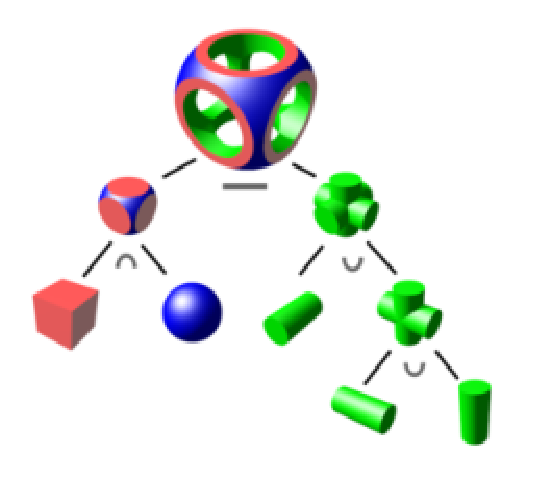
\includegraphics{csg_ex.eps}
  \caption{An example of how CSG volumes are created using Boolean combinations
    of smaller objects. The union of the three orthogonal cylinders is
    subtracted from the intersection of the box and sphere on the left to form
    the final volume at the top of the figure.}
  \label{fig:csg_ex}
\end{figure}

It is possible to construct complex geometries using CSG, but, as mentioned in
the introduction, the interface for this work is typically text-based and
defining complex volumes is a tedious and time-consuming task. Detecting
problems with the geometry definition is straightforward for the same reason
that particles can be robustly tracked through the geometry - the analytic
description of the surfaces. Fixing undefined regions of the geometry or
detecting invalid volume definitions is more difficult however.

The detection of intersections and particle containment queries in CSG
geometries is in practice computationally inexpensive for relatively simple
volume definitions, but due to the logical combinations of surfaces used to
create volumes the number of evaluations necessary to satisfy these queries is
linear with the number of surfaces in the definition. For sufficiently large and
complex models, it is not uncommon for volumes with many surfaces to be
artificially separated by planes to create two volumes with fewer surfaces in
their definition.

Visualization of CSG models can also be difficult. Because native formats for
CSG differ greatly between each Monte Carlo code, each typically comes with its
own visualization tools. These tools are typically restricted to 2D images of
the model representing a user-specified slice through the geometry. Other tools
such as MCAM \cite{Liu_2005} and McCad \cite{Tsigetamirat_2008} allow for
interactive visualization and repair of CSG models they do not provide the
accuracy of CAD modeling engines.

\subsection{CAD Geometry}

CAD systems allow for highly efficient and accurate geometric
representation. Highly complex models can be created using interactive
visualization tools represented in 3D space with a rich tool set for volume and
surface creation. These tools and the immediate visual verification of a user's
work reduces human error in model generation and design iteration.

In addition to reducing human error, CAD models provide a common domain for
analysis in other engineering domains such as fluid dynamics, heat transfer,
and structural engineering. This shared domain creates a common domain for
coupled physics simulation.

CAD also has the ability to represent free-form or higher-order surface. The use
of representations like splines and subdivision surfaces allow for more accurate
representation.

\subsection{Monte Carlo Radiation Transport on CAD Geometry}

The Direct Accelerated Geometry Monte Carlo (DAGMC) toolkit is a software
capable of Monte Carlo radiation transport directly on CAD models
\cite{Tautges_2009}. DAGMC was developed at the University of Wisconsin -
Madison. It has been coupled with many Monte Carlo codes to enable analysis on
CAD models. DAGMC relies on Cubit (and its commercial counterpart, Trelis) for CAD
modeling. Both of these CAD packages rely on the geometric modeling kernel,
ACIS.

DAGMC provides robust particle tracking for Monte Carlo transport on
arbitrarily complex CAD geometries. It accomplishes this by discretizing CAD
surfaces into sets of triangles. Volumes are then defined by any triangles which
represent bounding surfaces of a given volume. This surface mesh and the
geometric relationships between the mesh entities are stored in the Mesh
Oriented dAtaBase (MOAB) \cite{Tautges_2004}. These relationships are stored in
a hierarchical structure within MOAB, relating volumes to their surfaces,
surfaces to curves, and curves to vertices. 

It is important that geometric relationships of the mesh are maintained to
accelerate certain geometric queries on the surface mesh. For example,
\textit{Next Volume} queries are accelerated by using these relationships to
directly determine which volume a particle is passing into upon crossing a
surface rather than performing a query of the particle's location for each
volume. Other queries become more complicated due to the sheer number of
triangles needed to properly define volumes with detailed features. 

Next surface and closest to location geometry queries, for example, can be very
computationally expensive for volumes composed of hundreds of thousands or even
millions of triangles. A convenient way to think about performing geometric queries on
triangulated surfaces or volumes is to consider an equivalent CSG representation
constructed using a series of intersecting planes in place of triangles. The
structure imposed by the Boolean combinations used to define such volumes
require that each surface be checked for an intersection with the particle
trajectory. The nearest of these intersections can then be used to determine a
particle's crossing or movement to the physics event location specified by the
attached Monte Carlo code.

The problem of finding in intersection of a given particle location and
trajectory with a set of geometric primitives is known as ray tracing and is
well-studied in the field of computer graphics and animation. In this field,
data structures designed to accelerate the location of the nearest ray
intersection are applied.

\section{Ray Tracing Acceleration Data Structures}

Acceleration data structures for ray tracing are designed to rapidly narrow the
search for an intersection in virtual space given a starting position and
direction also known as a ray. This is accomplished by partitioning the space
and associating geometric primitives, most commonly triangles, with that
bounding partition. A search is performed by checking for an intersection with
the bounding partition. If the ray does not intersect with the partition, then
the set of primitives associated with that partition can be removed from the
search. If the ray does intersect with the partition, then the set of associated
primitives must be checked for intersection. Because a single separation into
two spatial partitions is often not enough to increase search efficiency, this
partitioning process is performed recursively. The result is a tree structure in
which at the top of the tree partitions are associated other partitions, known
as child nodes, rather than primitives. At the bottom of the tree exists a set of
nodes called leaves which are associated with geometric primitives. 

The search for a ray intersection then becomes a traversal of the tree
in which the children of the root node are checked for intersection. If an
intersection is found with one or both of the nodes, then the corresponding child nodes 
are checked for intersection as well. This process is repeated until leaf nodes
are reached at which point primitives are checked for intersection. Knowing that
a ray which doesn't intersect with a bounding partition cannot intersect with
any of the primitives it contains, allows many primitives to be rapidly removed
from the search and the number of intersection checks with primitives limited to
a small few. This technique reduces the algorithmic complexity of the search
from a brute force, or linear, $O(log(N_{triangles})$ to an $O(\,
log(N_{primitives}))$ search. 

\subsection{Partition Splitting Heuristics}

There are two components that go into the creation of spatial
partitions. The first is the selection of a candidate splitting plane which is
used to separate entities into one partition or another. The second is
the evaluation of the ``cost'' of that split should it be used. This cost is an
estimate of how good or bad the split would be. Because there is no way to know
exactly how expensive or inexpensive a split will be for the particular
simulation at hand, heuristics are used to evaluate this cost and determine the
optimal splitting plane using limited information about the local tree. This
information is typically limited to the number of primitives and bounds of the
parent partition and resulting child partitions.

The two heuristics will be addressed here - the Entity Ratio Heuristic (ERH) and the
Surface Area Heuristic (SAH). The ERH uses only the resulting number of
primitives in each child node to determine the cost of a split. The philosophy
behind this heuristic is to maintain the expected $O(log(N_{triangles})$ cost of
a ray traversal by ensuring that primitives are split as evenly as possible from
parent to child node. A form of this heuristic is presented in
Eq. \ref{eq:ERH}. This heuristic is unitless and bounded by zero and
one. This makes is possible to set both an upper and lower bound on the
unacceptable cost and a ``good enough'' cost.

\begin{figure}[H]
\begin{equation}
\label{eq:ERH}
 C = \frac{|P_{R}-P_{L}|}{(P_{R} + P_{L})} 
\end{equation}
  \begin{align*}
    C - & \,final \, cost \, evaluation \\
    P_{L} - & \, primitives\, contained\, by\, the\, left\, child  \\
    P_{R} - & \, primitives\, contained\, by\, the\, right\, child \\
  \end{align*}
  \caption{An example of the entity ratio calcution for a binary tree.}
  \label{fig:ERH}
\end{figure}

The SAH applies spatial information as well as division of primitives to the
cost evaluation. The SAH uses the surface area of candidate child partitions
relative to the current partition's surface area as an approximation for the
probability that the child will be visited after the parent volume. The explicit
form of the surface area heuristic was introduced in 1987 by Goldsmith and
Salmon \cite{Goldsmith_1987} and later formalized by MacDonald and Booth in 1990
\cite{MacDonald_1990}. Its full form is found in Equation \ref{eq:SAH}.

\begin{figure}[H]
  \begin{equation}
    C =  C_{t} + \frac{SA_{L}}{SA_{P}} |P_{L}|C_{i} +  \frac{SA_{R}}{SA_{P}} |P_{R}|C_{i}
    \label{eq:SAH}
  \end{equation}
  \begin{align*}
    C_{t} - & \,cost\, of\, traversal\, to\, child\, nodes \\
    C_{i} - & \, cost\, of\, primitive\, intersection\, check\, \\
    SA_{L} - &  \,surface\, area\, of\, left\, child \\
    P_{L} - & \, primitives\, contained\, by\, the\, left\, child  \\
    SA_{R} - & \, surface\, area\, of\, right\, child \\
    P_{R} - & \, primitives\, contained\, by\, the\, right\, child \\
    SA_{P} - & \, parent\, bounding\, volume \\
  \end{align*}
  \caption{A form of the surface area heuristic for a binary tree.}
  \label{fig:SAH}
\end{figure}

For the general case, ERH has not proved to be as effective as the SAH, but it
has proven to be a useful tool in correcting the surface area heuristic for
triangle mesh features of a specific type. This scenario will be discuss further
in <INSERT HV CHAPTER HERE>.


\chapter{Geometry Query Preconditioning}\label{ch:preconditioning}

This chapter describes the adaptation of a rendering data structure, the signed
distance field, as a geometric query tool for accelerating CAD-based transport
in the Direct Accelerated Monte Carlo (DAGMC) toolkit. The beginnings of a
predictive model for the data structure's utilization based on various problem
parameters is also introduced and demonstrations of its effectiveness are shown
for a number of simple problems as well two production level models.

\section{Signed Distance Field Preconditioning}\label{section:preconditioner_theory}

Three types of geometric queries are common among the various Monte Carlo codes
that DAGMC supports. These include next surface intersection, point containment,
and closest boundary intersection queries. Typically, a ray is fired to satisfy
any of these queries in DAGMC with $O(logN)$ complexity, but it is hypothesized
that these queries can be accelerated in many cases by first performing an
$O(1)$ signed distance value look-up to precondition the higher complexity ray
fire calls and make sure they are necessary.

Point containment queries can be performed by examining the signed distance
value for the current particle location. If the point's value is negative (or
outside of the signed distance field data structure), then the point is not
contained within the volume. If the point's value is positive, then the point is
determined to be inside the volume. Given that there is error associated with
each of these interpolated values, the point containment using a signed distance
field should only be trusted if the absolute value of the signed distance is
greater than the expected error associated with the value. If this is not the
case, then a ray must be fired to determine the particle's containment with
respect to the volume in question.

Closest to boundary queries can be performed in a similar manner to the point
containment queries, but they are more dependent on the native code's intent for
their use. Some Monte Carlo codes query for the nearest volume surface
intersection in order to determine whether or not the particle will exit the
volume before reaching its next physics event location. Signed distance fields are
designed for exactly this operation. In similar fashion to the point
containment case, the signed distance value should only be trusted if it is greater than the
error associated with the value. Additionally, the error should be subtracted
from the value, returning to the code a conservative value for the nearest
intersection. If the signed distance value's magnitude is not greater than its
error evaluation or if the value is negative, then a ray should be fired to
determine the exact location of the nearest boundary crossing for the particle's
location.

Next surface intersections are called by native Monte Carlo codes to determine
if a particle will cross a surface before reaching its next physics event
location. This is the most common geometry query in an average Monte Carlo
simulation. Normally in DAGMC a ray is fired each time this query is
called. This can be avoided by using the signed distance field to exclude the
possibility of a surface crossing without explicitly determining the next
surface intersection. If the sum of the signed distance values for both the
current particle position and the next physics event location is greater than
the distance between the two, then no surface crossing will occur and the
particle can safely advance to the next physics event location. For robustness,
the error for each interpolation should be subtracted from the sum of the signed
distance values as a conservative measure. If the expanse between the particle's
current location and its next physics event interaction cannot be accounted for
by the signed distance values of the two points, then a ray will be fired to
determine the particle's next surface intersection along that
trajectory. Fig. \ref{fig:precondition_ray} shows a graphic representation of
this process. Not all Monte Carlo codes provide the next physics event location
along with the particle's current location to their geometry kernels. In this
case, preconditioning of these queries will not be possible.

\begin{figure}[ht]
  \center
  \includesvg{../images/preconditioner_ex}{0.35\textwidth}
  \caption{Visualization of ray preconditioning scenarios. The $\epsilon$ here represents
    the associated error of the signed distance value interpolation.}
  \label{fig:precondition_ray}
\end{figure}

Using these methods, the storage of signed distances field for volumes in DAGMC
could provide a way to accelerate the Monte Carlo queries listed above by using
a $O(1)$ process to establish that the conditions of a geometric query are such
that a more robust and computationally expensive ray is necessary before
performing the ray tracing operation. It is hypothesized that in many cases
during radiation transport that this process can be used to subvert many ray
tracing calls and a large number of these $O(logN)$ searches can be avoided.

\begin{figure}[ht]
  \includesvg{../images/preconditioner_datastruct}{0.3\textwidth}
  \centering
  \caption{2D visualization of the signed distance field with sign conventions reversed for use in radiation transport.}
  \label{fig:preconditioner_datastruct}
\end{figure}

\section{Signed Distance Field Implementation in DAGMC}

\subsection{Construction}

An initial implementation of the signed distance field employed MOAB's
structured mesh interface and data tagging capabilites for storage of the data
structure. This interface maintains a representation of the structured mesh with
vertex coordinates and handles at each point along with hex elements for each
mesh voxel. These vertex coordinates and hex elements can be accessed using
$<i,j,k>$ indexing. While this format is somewhat memory intensive, it provides
a fast path for verification, visualization, and proof of concept in transport
test cases for demonstration.

\begin{figure}
  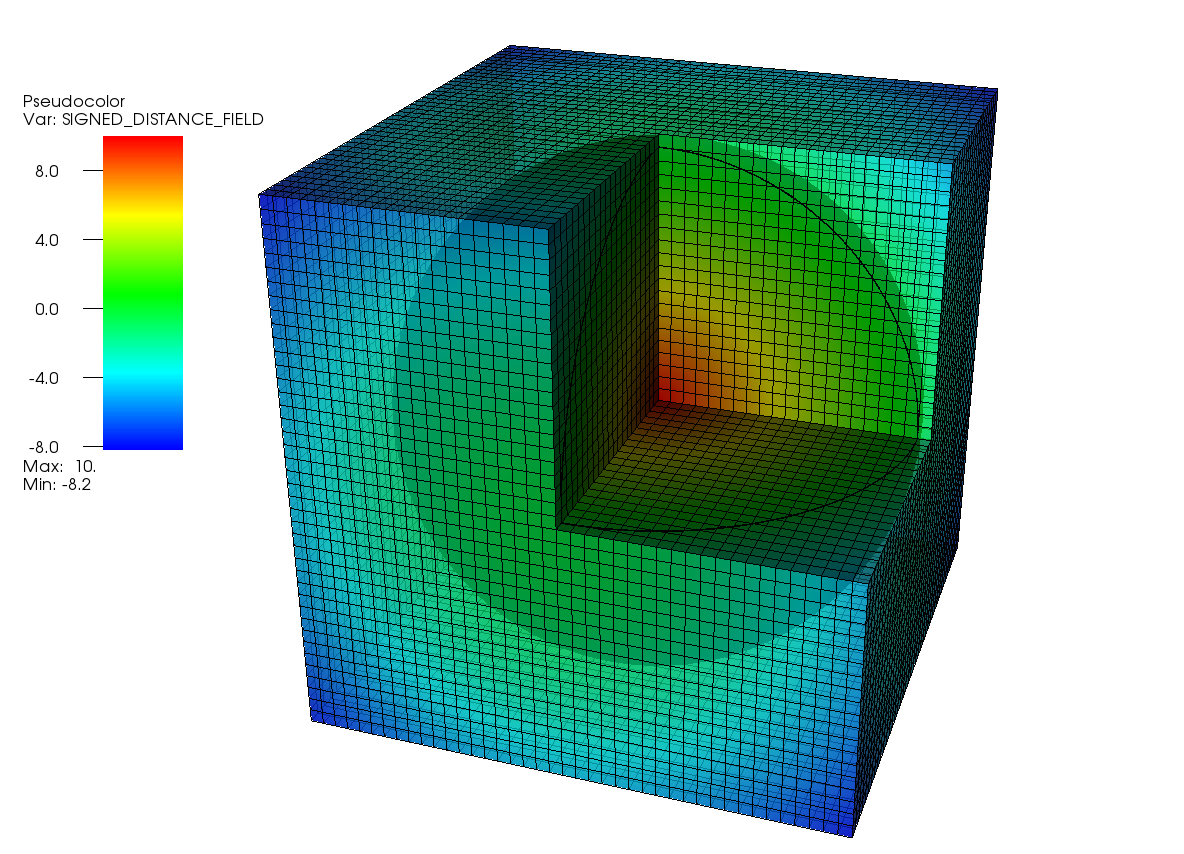
\includegraphics[scale=0.22]{../images/sdf_sphere.png}
  \caption{A visual of a signed distance field with step size 0.5 cm surrounding
    the spherical volume of test case with a radius of 10 cm.}
  \label{fig:sdf_sphere}
\end{figure}

Signed distance values can be retrieved from the structured mesh by determining
which mesh voxel the point lies within. The point's element is accessed by
determining an $<i,j,k>$ index using the point's x, y, and z values divided by
the structured mesh step size. A trilinear interpolation of the element's 8 vertex
coordinates and their signed distance values is then used to provide the signed
distance value for the location of interest. As a result, the complexity of a
signed distance value lookup from the signed distance field is
$O(1)$. Performance improvements for geometric queries are based on using this
process in place of the $O(log(N))$ ray tracing process.

A much less memory intensive implementation in which only a box
corner, grid step size, dimensions, and the signed distance value data are
stored has now also been implemented. This avoids the storage of vertex
coordinates, mesh element connectivity, and all associated handles to those
entities. There is an added cost in re-computing vertex coordinates when a
signed distance value is interpolated, but this added cost should still be
negligible in comparison to a ray traverval and memory is of greater concern for
this spatially dense data structure. This data structure can still interact with
MOAB's structured mesh interface to generate an explicit mesh for visualization
and verification if required.

As an initial implementation, one signed distance field is generated for each
volume in DAGMC with extents matching the axis-aligned bounding box of the
volume. The signed distance field is represented as a uniform structured mesh
with a signed distance value at each vertex in the mesh as indicated in Fig.
\ref{fig:preconditioner_datastruct}.\footnote{Altering the sign convention when
  populating the data structure rather than incurring the additional
  computational cost of altering the sign of values for each operation is
  preferable.}

\subsection{Population}

It is mentioned above that signed distance fields are typically
generated using an implicit, analytic representation, but a suitable data
structure for populating the structured mesh with signed distance values is
already in place in the form of DAGMC's bounding volume hierarchy. It is a more
straightforward process to simply use DAGMC's current closest to location
algorithm to generate signed distance values than to create an implicit surface
approximation of the triangle mesh. Though the latter may be faster,
performance improvements didn't seem to be impeded greatly by using this method
to populate the data structure. This method also maintains a consistency between
the intersections found by the ray tracing kernel and the signed distance field
values.

DAGMC's closest to boundary algorithm returns, among other pieces of
information, the nearest intersection location and the triangle on which this
intersection exists. For each point in the signed distance field mesh, this
algorithm is used to determine the magnitude of the distance value. To determine
the sign of the distance value, a ray is constructed from query location and the
intersection location. The dot product of this ray vector with the triangle's
outward normal vector is used to determine the sign of the distance value. DAGMC
maintains enough information to consistently orient triangle normals such that
they point outward from the volume they represent. In the rare cases for which
the dot product of these vectors is ambiguous, or zero, DAGMC's point
containment algorithm is used to disambiguate the value's sign.


\section{Signed Distance Field Utilization}\label{section:preconditioner_utilization}

In effect, the preconditioner is attempting to check whether or not the particle
will actually cross a surface before explicitly searching for the particle's
intersection with a surface along its current trajectory. If the result of this
preconditioning check is always false and a ray is always fired, then these
checks are only adding to the computational cost of the problem. This will
always occur in volumes filled with void, for example, as particles immediately
travel from one surface to another. As a result, the signed distance field
should be applied selectively depending on each volume's geometric and material
properties for optimal performance and high utilization of the preconditioning
methods. Ideally, this method will only be applied to volumes in which the data
structure is able to precondition ray fire calls often or with high utilization
of the data structure. The signed distance field is expected to have the biggest
impact in performance when preconditioning next surface intersection queries, as
they are most frequently called in Monte Carlo codes when tracking particles
through the geometry. As such, this type of query is the focus of utilization
measurement for the remainder of this section.

\begin{equation}
  U = \frac{ \small \text{Rays Avoided w/ SDF} }{ \small \text{Number of Geometry Queries} } 
   \label{eq:preconditioner_utilization}
%  \caption{Definition of signed distance field utilization as a ray fire preconditioner in DAGMC.}
\end{equation}

The utilization, $U$, of the signed distance field as a ray fire preconditioner can be
described as the number of rays fire calls related to the next surface
intersection queries that are avoided divided by the total number of next surface
intersection queries made by the Monte Carlo code. This value is described
in Eq. \ref{eq:preconditioner_utilization} and can be quantified using this
definition using debugging tools, such as Valgrind, during DAGMC simulations.
It is expected that in the majority of cases, as the utilization of preconditioning
methods goes up, the performance of the simulation will also improve.

\begin{figure}[ht]
  \centering
  \includesvg{../images/sdf_hydrogen_density_study_perf}{0.5\textwidth}
  \caption{Performance results for a 5 MeV neutron source at the origin of a 10
    cm radius sphere. Hydrogen density was varied from 0 to 1
    $\frac{g}{cm^3}$. Simulations of 100M histories at each density were
    performed using native MCNP5, DAG-MCNP5 without the signed distance field,
    and DAG-MCNP5 with the signed distance field.}
  \label{fig:sphere_hydrogen_density_study_perf}
\end{figure}

To understand this utilization more deeply with respect to material parameters,
the hydrogen density was varied from 0 to 1 $\frac{g}{cm^3}$ in the single-volume
sphere test problem with a 5 MeV neutron point source. For each density, one
simulation was performed without the signed distance field and another with the
signed distance field and preconditioning enabled. Fig.
\ref{fig:sphere_hydrogen_density_study_util} shows the results of this study. 

\begin{figure}[ht]
  \centering
  \includesvg{../images/sdf_hydrogen_density_study_util}{0.5\textwidth}
  \caption{Utilization results for a 5 MeV neutron source at the origin of a 10 cm radius
    sphere. Hydrogen density was varied from 0 to 1 $\frac{g}{cm^3}$.}
  \label{fig:sphere_hydrogen_density_study_util}
\end{figure}

Utilization of the data structure in this study remains high until the hydrogen
density falls to 0.1 $\frac{g}{cm^3}$ at which point a distinct knee appears and
the utilization falls off quickly. Even at the lowest density reached in the
study of 0.01 $\frac{g}{cm^3}$, the utilization of the signed distance field to
avoid ray fire calls is 0.54.  It is difficult to judge the impact on the
performance of this simulation for these low density values due to the limited
size of the geometry and the short lived histories. As the material density
decreases, particles quickly leave the geometry after very few collisions, but
Fig. \ref{fig:sphere_hydrogen_density_study_perf} provides an impression of the
performance of these three implementations converge as the density of the
hydrogen is varied. The application of the signed distance field allows for
significantly improved performance until the density drops below 0.1
$\frac{g}{cm^3}$ in agreement with utilization plot. In order to have more
control over a simulation's physical parameters, subsequent experiments were
performed using a simple simulation tool.

\section{Signed Distance Field Utilization Modeling}

In order to characterize utilization of a signed distance field as a next
surface intersection query preconditioner for ray fire calls in DAGMC, a pseudo
Monte Carlo simulation tool was developed using DAGMC. This tool was used to
simulate different transport scenarios within a spherical geometry using an
isotropic volumetric source and isotropic scattering. Particle histories are
terminated based on a maximum number of collisions or departure from the problem
geometry. Particle distance traveled, $d$, can be represented by either a fixed
distance or by sampling for the standard probability of interaction in a medium
with mean free path, $\lambda$. The tool allows the mean free path to be set
directly, enabling a relation between the signed distance field and this value
to be developed with the intent to use this relationship as a means for
characterizing appropriate conditions for application of the signed distance field.

\begin{figure}[!htb]
  \centering
  \includesvg{../images/sdf_fixed_dist_results}{0.5\textwidth}
  \caption{Results of the model for the theoretical utilization limit with the
    results of the simulation for a fixed distance traveled case.}
  \label{fig:sdf_fixed_dist}    
\end{figure}

To begin, simulations were performed for particles with a fixed distance
traveled, $\lambda$, varying that distance and the
signed distance field step sizes. Run times of the simulation are not shown here
as the data structure's utilization is the main focus of this study. The results
of this study are shown in Fig. \ref{fig:sdf_fixed_dist}. As the signed distance
field mesh step size increases, utilization of the data structure decreases due
to the increasing error associated with the interpolation of signed distance
values. Additionally, utilization is expected to decrease with increasing
distance traveled. This decreased utilization is caused by not only the increased
distance between the two particles, but also by the increased probability
that both locations will be closer to surfaces of the sphere and have smaller
signed distance values. A theoretical limit for the utilization is also shown in
Fig. \ref{fig:sdf_fixed_dist}. The development of the analytic form for this limit will now be
discussed.

\begin{figure}[ht]
  \centering
  \includesvg{../images/alpha}{0.3\textwidth}
  \caption{Depiction of model variables.}
  \label{fig:model}
\end{figure}

The utilization of the signed distance field as a preconditioner for ray tracing
operations can be modeled as an evaluation of the combined probability space for
particles with a current position, $\vec{p}$, and a next physics event location,
$\vec{n}$, after traveling a distance, $d$. The fraction of this probability
space in which signed distance values can be used to rule out surface crossings
for next surface intersections is then considered to be the theoretical
utilization of the signed distance field. An initial form for this probability
space can found in Eq. \ref{eq:util_model}.

\begin{equation}
  \label{eq:util_model}
\int_{V_{sphere}}\int_{V_{track}} p_p(r) p_n(d) \, \mathrm{d}V_{sphere}\mathrm{d}V_{track}
\end{equation}

In this model, the starting location of particles, $\vec{p}(r,\phi,\theta)$, is
uniformly distributed, $p_p(r)=1$, throughout a sphere of radius, $R$.  The
location of the next event, $n(d,\alpha,\beta)$, where $d$ is the distance
traveled by the particle, $\alpha$ is the interior angle between the
particle's \textit{position} vector and the particle's sampled direction
vector, and $\beta$ represents an azimuthal angle for directions traveled with
angle of departure $\alpha$. Fig. \ref{fig:model} depicts these
variables, $r$, $d$, and $\alpha$ more clearly.  These points are distributed
uniformly on a sphere at some distance $d$, and that distance is distributed
according to some probability density function, $p_n(d)$. 

In Eq. \ref{eq:util_model} the outer integral represents all possible particle positions within the
geometric sphere and expands to

\begin{equation}
\int_{0}^{R}\int_{0}^{2\pi}\int_{0}^{\pi}\int_{V_{track}} r^2\sin{\phi} \, \mathrm{d}\phi
\mathrm{d}\theta \mathrm{d}r \,  p_n(d) \mathrm{d}V_{track}
\end{equation}

The second integral then expands to

\begin{equation}
\small \int_{0}^{R}\int_{0}^{2\pi}\int_{0}^{\pi}\int_{0}^{\infty}\int_{0}^{2\pi}\int_{0}^{\pi}
r^2\sin{\phi} \, p_n(d) d^2 \sin{\alpha} \, \mathrm{d}\alpha \mathrm{d}\beta \mathrm{d}d \, \mathrm{d}\phi
\mathrm{d}\theta \mathrm{d}r
\end{equation}

Integration of $\phi$, $\theta$, and $\beta$ can now be performed with
the knowledge that they are symmetric with respect to the problem and
integration of $p_n(d)$ does not rely on them.

\begin{equation}
\small 8\pi^2  \int_{0}^{R}\int_{0}^{\infty}\int_{0}^{\pi} p_n(d) \,
r^2 \, d^2 \sin{\alpha} \, \mathrm{d}\alpha \mathrm{d}d \, \mathrm{d}r
\end{equation}

In order to represent particles traveling a fixed distance, the relationship in Eq. \ref{eq:pn_fixed}
is applied.

\begin{equation}
  \label{eq:pn_fixed}
  p_n(d) = \frac{\delta(d-\lambda)}{d^{2}}
\end{equation}

The evaluation of this integral then gives a representation of all the query
space available to the problem

\begin{equation}
  \label{eq:A_fixed}
\small A = 8\pi^2  \int_{0}^{R}\int_{0}^{\infty}\int_{0}^{\pi} \delta(d-\lambda) \,
r^2 \, \sin{\alpha} \, \mathrm{d}\alpha \mathrm{d}d \, \mathrm{d}r
\end{equation}

and represents all geometric query space, $A$, for a sphere of radius,
$R$ and a fixed distance traveled, $\lambda$.

In order to understand what fraction of this query space is able to be
preconditioned, the condition for avoiding an explicit nearest intersection
search along a particle direction in Eq. \ref{eq:condition} must now be
applied. Because this is intended to be an idealized upper limit for the
utilization, error will be ignored.

\begin{equation}
  SDV(\vec{p}) + SDV(\vec{n}) > |\vec{p}-\vec{n}| + 2\varepsilon(h)
  \label{eq:condition}
\end{equation}
\begin{align*}
 &SDV - \, signed \, distance \, value \, function \\
 &\vec{p} - \, particle's \, current \, position \\
 &\vec{n} - \, particle's \, next \, event \, location \\
 &h - \, mesh \, step \, size \\
 &\varepsilon(h) - \, error \, evaluation \, for \, signed \, distance \, values \\
\end{align*}

This condition establishes that the nearest location to intersection for both
points must be greater than the distance between the two points plus any error
associated with their signed distance values as previously discussed. This
condition is true for some fraction of the next surface queries in a Monte Carlo
simulation, but not all.  Our mathematical model has no error, allowing for the
largest possible volume of locations in which preconditioning will apply and the
signed distance value for any point, $\vec{x}$, is

\begin{equation}
SDV(\vec{x}) =  R-|\vec{x}|
\end{equation}

Making these substitutions into the inequality gives

\begin{equation}
R-|\vec{p}| + R - |\vec{n}| >   |\vec{p}-\vec{n}|
\end{equation}
The right hand side of this inequality can simply be described as the distance
traveled, $d$, and the magnitude of $\vec{p}$ can be represented
by the variable $r$.

\begin{equation}
 R-r + R - |n(d,\alpha,\beta)| > d
\end{equation}

Reducing the next event location, $\vec{n}(d,\alpha,\beta)$, into an expression
in terms of $r$, $d$, and $\alpha$ requires further examination of the
problem. Because the coordinates of $n$ depend on the current particle position,
the magnitude of $n$ with respect to the geometry origin must be obtained to get
a correct form for the signed distance value. Again, Fig. \ref{fig:model} depicts the
value of $n$ graphically for reference. The magnitude of n can then be described
using the law of cosines as

\begin{equation}
|n(d,\alpha,\beta)| = \sqrt{r^2 + d^2 - 2rd \cos{\pi-\alpha}}
\end{equation}
inserting this into the inequality gives

\begin{equation}
R-r + R - \sqrt{r^2 + d^2 + 2rd \cos{\alpha}} > d
\end{equation}

The inequality has now been reduced to the three variables seen in
Eq. \ref{eq:A_fixed} ($r$,$d$, and $\alpha$). This inequality can be applied to
construct limits of integration representing boundaries of space in which the
SDF can be utilized. By rearranging the inequality, a limit on the angle of
departure, $\alpha$, from the particle's position can be derived.

\begin{equation}
\alpha_{min} > \arccos\Bigg ( \frac{(2R-r-d)^2-d^2-r^2}{2 d r} \Bigg )
\end{equation}

\begin{figure*}[ht]
  \centering
  \includesvg{../images/model_cases_fixed_distance}{0.8\textwidth}
  \caption{Depiction of modeling cases.}
  \label{fig:modeling_cases}
\end{figure*}

This condition on alpha can be interpreted as a minimum interior angle that the
particle's trajectory must take relative to the particle's position vector,
$\vec{p}$, for a distance traveled, $d$, for a ray fire to be avoided and the
preconditioner to be utilized. The examination of this condition as a function
of the distance traveled for various values of $r$ results in some conclusions
about how signed distance values are being utilized.

\begin{figure}
\centering
\includesvg{../images/alpha_r}{0.5\textwidth}
\caption{Plot of minimum angle of departure restriction for particles with
various radial positions in a sphere with R = 100 cm and varying distances traveled.}
\end{figure}

The inequality is undefined until the distance reaches a value $d = R- r$. This
is because the angular limit only needs to be applied to areas of the query
space in which the distance traveled is large enough to violate the above
condition as depicted in Fig. \ref{fig:modeling_cases}. A violation of this
limit may only occur when a particle travels far enough to reach the geometric
sphere boundary along the current position vector as if it were moving directly
toward the boundary of the sphere. An additional interesting feature of this
plot is the convergence of all the curves as $d \rightarrow R$ on $\pi$. The
convergence on $\pi$ indicates that as the distance traveled approaches $R$ the
only direction that the particle can move is back toward the origin along the
position vector. It also defines a maximum distance a particle can travel in the
sphere and still be preconditioned using signed distance values. Intuitively
this makes sense as the maximum chord length of a sphere is $2R$, and once a
particle travels a distance $R$ the sum of the signed distance values can then
be no larger than $R$ and the condition for utilization in Eq. \ref{eq:condition} is
violated. Hence all curves go to zero at $\lambda = 100 cm$ in
Fig. \ref{fig:sdf_fixed_dist}.

In order to account for the fact that the form of $\alpha_{min}$ is undefined
until $d = R-r$, a Heaviside function is applied before applying it as a limit
on the particle's angle of departure from the position vector. Similarly,
because the $\alpha_{min}$ condition is undefined after $d=R$ a Heaviside
function is used to limit the condition to $\pi$ for any distances traveled
larger than $R$.

\begin{equation}
  \small
  \begin{split}
  \alpha_{min} =& (H(d-(R-r))-H(d-R)) \arccos\Bigg ( \frac{(2R-r-d)^2-d^2-r^2}{2 d r} \Bigg ) \\
  &+ \pi \, H(d-R)
  \end{split}
\end{equation}


By inserting this condition as a lower limit of the $d\alpha$ integration, the
following integral will give all utilized space, $US$, in the query space of the
simulation.

\begin{equation}
  \label{eq:subs_a_cond}
\small US = 8\pi^2  \int_{0}^{R}\int_{0}^{\infty}\int_{\boldsymbol{\alpha_{min}}}^{\pi} \delta(d-\lambda) \,
r^2 \, d^2 \sin{\alpha} \, \mathrm{d}\alpha \mathrm{d}d \, \mathrm{d}r
\end{equation}

Evaluating this integral and dividing by all query space gives the
following form for the theoretical limit of signed distance field utilization as a
preconditioner for ray firing

\begin{equation}
U_{theoretical} = \frac{US}{A} =  \frac{(1-H(\lambda-R))(2R-\lambda)(R-\lambda)}{2R^2}
\end{equation}

It can be seen in Fig. \ref{fig:sdf_fixed_dist} that this utilization limit
works well as an upper limit for the simulation results using various signed
distance field mesh resolutions. As the step size of the mesh approaches zero,
so does the evaluation of the error, resulting in the same utilization curve
with varying distance traveled, $\lambda$, as in the analytic form developed
here. Future work will include the comparison of this utilization limit to other
single-volume geometries using dimensionless parameters to determine if the
model above can be used to predict signed distance field utilization in other
geometries as well.

With the agreement of the simulation results and analytic model for signed
distance field utilization for the fixed distance traveled case, the simulation
has been used to produce a similar set of results in which the distance is
sampled based on the standard probability for distance to interaction in a
medium with a cross section, $\Sigma$, or mean free path $\lambda
=1/\Sigma$. This results in the probability distribution function shown in
Eq. \ref{eq:pn_sampled} for the particle distance traveled in this scenario.

\begin{equation}
  \label{eq:pn_sampled}
p_n(d) \propto \frac{e^{-\Sigma d}}{d^{2}} = \frac{e^{-\frac{d}{\lambda}}}{d^{2}}
\end{equation}

\begin{figure}[ht]
\centering
\includesvg{../images/sdf_sampled_dist_results}{0.5\textwidth}
\caption{Results of the model for the theoretical utilization limit with the
results of the simulation for a sampled distance traveled case.}
\label{fig:sdf_sampled_dist}
\end{figure}

%has to be in this section for latex reasons. grumble grumble...
\begin{table*}[!h]
  \centering
  \begin{tabular}{lcccc}
          \multicolumn{5}{l}{\textbf{\textit{Source Location:}} <0,0,-1>} \\
          \textbf{Implementation} & \textbf{ctme (min)} & \textbf{wall time
            (min)} & \textbf{time ratio} & \textbf{precond. utilization}\\
          \hline
          MCNP6 & 0.17 & 0.14 & 1 & N/A \\
          DAG-MCNP6 & 1841.33 & 1841.33 & ~11,000 & N/A \\
          DAG-MCNP6 w/ SDF & 0.48 & 0.46 & 2.82 & 0.94\\
          \multicolumn{5}{l}{} \\
          \multicolumn{5}{l}{\textbf{\textit{Source Location:}} <0,0,10>} \\
          \textbf{Implementation} & \textbf{ctme (min)} & \textbf{wall time
            (min)} & \textbf{time ratio} & \textbf{precond. utilization}\\
          \hline
          MCNP6 & 0.18 & 0.18 & 1 & N/A \\
          DAG-MCNP6 & 11.12 & 11.16 & 62 & N/A \\
          DAG-MCNP6 w/ SDF & 0.50 & 0.52 & 2.89 & 0.96 \\
          
  \end{tabular}
  \caption{Performance results for an MCNP6 test case involving electron
    transport of a 1 keV-100 keV photon source incident on an Fe/W target. 5,000
    histories were run in this test problem.}
  \label{tab:inp066_results}
\end{table*}

Following the same process as in the fixed distance case by plugging Eq. \ref{eq:pn_sampled} into
Eq. \ref{eq:subs_a_cond}, the utilization form for the sampled distance case is
shown in Eq. \ref{eq:sampled_limit}.

\begin{equation}
  \label{eq:sampled_limit}
  U_{theoretical} = \frac{US}{A} = \frac{ \frac{1}{2} \lambda(R - 2 \lambda) e^{\frac{-R}{\lambda}} + \lambda^2 - \frac{3}{2} R \lambda + R^2 }{R^2}
\end{equation}

The results of this set of simulations can be seen in
Fig.\ref{fig:sdf_sampled_dist}. In this scenario, it is not expected that the
utilization will approach zero when $\lambda = 100\, cm$, as the actual distance
sampled may be considerably less than the provided mean free path for the
simulation. Overall utilization values in this scenario for $\lambda$ from 0 to
100 cm remain higher than the corresponding fixed distance simulation cases as
is expected in a sampled distance case. Utilization values remain high for
relatively large increases in mesh step size, $h$. This is important to
application of the data structure given concerns regarding its potentially high
memory footprint for large volumes. For example if the utilization of the signed
distance field drops $~20\%$ when going from a step size of 1 cm to 6.21 cm, but
the memory footprint of the data structure will have decreased by a factor of
$6.21^3$ or $239.5$ as well. The optimization of the mesh step size with respect
to its effect on utilization will also need to be included in future models of
the utilization.

The fixed distance traveled scenario provides a nice baseline for agreement
between the computational results and the model, but a more realistic scenario
is required before attempting to apply the model as a predicitive utility for
application of the SDF in true Monte Carlo codes. The most useful alteration of
the current simulation scenario is to move from a fixed distance distance to a
sampled distance based on the standard probability for distance to interaction
in a medium given a cross section, $\Sigma$.

$$ p = e^{-\Sigma d} = e^{-\frac{d}{\lambda}} $$

where in this case now $\lambda$ represents the mean free path of the particle in the medium

In simulation, distances are now sampled as

$$ d = -\lambda ln(p) $$

where p is randomly sampled with a uniform distribution between 0 and 1

Inserting this definition for the particle distance into the integrals above
gives

$$ \frac{dp}{dd} = -\frac{p}{\lambda} $$
$$ d = 0 \rightarrow p = 1 $$
$$ d = D \rightarrow p = 0 $$

$$ \int_{0}^{R}\int_{0}^{2\pi}\int_{0}^{\pi}\int_{1}^{0}\int_{0}^{2\pi}\int_{0}^{\pi}
-r^2\sin{\phi} \, \lambda p ln(p)^2 \sin{\alpha} \, \mathrm{d}\alpha \mathrm{d}\beta \mathrm{d}p \, \mathrm{d}\phi
\mathrm{d}\theta \mathrm{d}r $$

This integral can then be evaluated to give the entirety of the geometry space
for the problem

\begin{center}
All Query Space = $\frac{4}{3} \lambda \pi^2 R^3$
\end{center}

To find the portion of utilized space for a given $R$ and $\lambda$ one can
apply the same methods from the fixed distance case, for each particle position
within the sphere there will still be two scenarios - one in which the distance
traveled exceeds $R-d$ and another in which it is less than $R-d$. The difference
now is d has become a distrubution rather than a constanct value, so as the
distance traveled changes the queries will fall into either category for a
single particle position.


Another way of viewing of viewing this condition in the case of a varying
distance is to define these same categories based on the distance traveled. Now
rather than defining how the angular condition is applied based on position, the
angular condition will be applied based on the distance the particle travels.


$$ d < R-r : \alpha_{min} = 0 $$
$$ d > R-r : \alpha_{min} = \arccos\Bigg ( \frac{(2R-r-d)^2-d^2-r^2}{2 d r} \Bigg
) $$

It is interesting to examine plots of the angular limit with varying distance as
seen in Fig. \label{fig:alpha_min}

\begin{figure}[ht] \label{fig:alpha_min}

\centering
\includesvg{alpha_r}{1\textwidth}
\caption{Plot of mininum angle of departure restriction for particles with
various radial positions and varying distances traveled.}
\end{figure}

The entry point of each curve in the plot represents the minimum distance
necessary to enter the $d > R-r$ region and begins to apply an agular
restriction. Note that each of these approach a mininmum angle of $\pi$ as the
distance traveled approaches $R$ (100cm). This represents a particle traveling
back towrd the origin along the sphere's larges chord with length $2R$ and,
again,the maximum distance a particle can travel before the SDF can no longer be
utilized.

Now that the distance traveled is being used to construct these two regions in
the model, this integral must be separated into two pieces, one with limits of $0$
to $R-r$ and another with limits $R-r$ to $R$. Based on the distance sampling
distribution, these values become

$$ d_{min} = R-r \rightarrow p_{max} = e^{(-\frac{(R-r)}{\lambda})} $$
$$ d_{max} = R   \rightarrow p_{min} = e^{(-\frac{R}{\lambda})} $$

and our integral becomes

$$ \int_{0}^{R}\int_{0}^{2\pi}\int_{0}^{\pi}\int_{1}^{p_{max}}\int_{0}^{2\pi}\int_{0}^{\pi}
-r^2sin(\phi) \, \lambda p ln(p)^2 sin(\alpha) \, \mathrm{d}\alpha \mathrm{d}\beta \mathrm{d}p \, \mathrm{d}\phi
\mathrm{d}\theta \mathrm{d}r + $$
$$ \int_{0}^{R}\int_{0}^{2\pi}\int_{0}^{\pi}\int_{p_{max}}^{p_{min}}\int_{0}^{2\pi}\int_{alpha_{min}}^{\pi}
-r^2\sin{\phi} \, \lambda p ln(p)^2 \sin{\alpha} \, \mathrm{d}\alpha \mathrm{d}\beta \mathrm{d}p \, \mathrm{d}\phi
\mathrm{d}\theta \mathrm{d}r $$

The evaluation of this integral divided by the full geometry query space for the
distance sampling scenario after the $c=\frac{R}{\lambda}$ replacement is

$$U(c) = \frac{1}{4}\frac{(4 c^2-6) c^2e^{-2c} - (c^3-c^2-\frac{3}{2}
c+3)4ce^{-2c}+(-2 c^3+2c^2+9c-6) e^{-2c}+4c^2-9 c+6}{c^2}$$

\begin{figure}[ht] \label{fig:sdf_sampled_dist}
\centering
\includesvg{sdf_sampled_dist_results}{\textwidth}
\caption{Results of the model for the theoretical utilization limit with the
results of the simulation for a fixed distance traveled case.}
\end{figure}

Unfortunately the predictive model for the sampled distance scenario is not
consistent with the simulation results, and under predicts the utilization of
the SDF significantly. It is quite possible that utilization in either th interior or exterior
resion of the sphere is being under represented. Regardless of the cause, examining the contribution to
utilization from each of these regions (shown in
Fig. \label{fig:util_region_contributions}) is an interesting endeavor.


\begin{figure}[ht] \label{fig:util_region_contributions}
\centering
\includesvg{../images/util_contributions}{\textwidth}
\caption{A plot of the total predicted utilization along with the contriubtions
from the inner region ($d < R-r$) and outer region ($d > R-r$).}
\end{figure}

When the mean free path $\lambda$ is very small, particles' next event locations
rarely reach the outer region condition. As $\lambda$ increases, particles are
more likely to enter that region and its contribution increases greately. Then
as particles begin to travel distances on the order of the sphere radius the
utilization decreases. The interior region utilization acts as one would
expect. When particles travel small distances with respect to the sphere radius,
there is high utilization, but as the particles begin to travel further its
utilization rapidly decreases. The contribution from the outer region defines the
significance of using both the current position signed distance value as well as the
next event location's signed distance value to precondition ray fire calls in DAGMC.


% 
\section{Motivation}

\begin{frame}
  \frametitle{CAD-Based Monte Carlo}
\end{frame}

% \include{related/related}

%% etc, etc.

%% Do you have appendices?  If so, add them here, just like chapters.
% \begin{appendices}
% \include{backmatter/appendix1}
% \end{appendices}

%% Are you a big nerd with a colophon?  Add it here.
\begin{colophon}
\svnidlong{$LastChangedBy$}{$LastChangedRevision$}{$LastChangedDate$}{$HeadURL: http://freevariable.com/dissertation/trunk/frontmatter.tex $}
\vcinfo{}

This template uses Gyre Pagella by default.  (I used Arno Pro in my dissertation.)

Feel free to give me a shout-out in your colophon or acks if this template is useful for you.  Good luck!

\end{colophon}

%% McBride is a very nice style (some version is included in this distribution)
\bibliographystyle{mcbride}
\bibliography{refs}

%% Want an index?  Neither did I.
%\printindex

\end{document}
